\documentclass[12pt]{article}

%------------------------------------------%
%                Packages 
%------------------------------------------%
%These are the packages that we will use in our latex document. 

\usepackage{graphicx}
\usepackage{natbib}	%Bibliography package. It handles citations and can easily change formats. This is done at the end of the document
\usepackage[utf8]{inputenx}% For proper input encoding
\usepackage{adjustbox} %Handles resizing of tables, figures, etc. Based off of page and/or line width/height 
% Packages for tables
\usepackage{booktabs}% For Pretty tables
\usepackage{threeparttable}% For Notes below table
\usepackage{rotating}% To Rotate Table
\usepackage{amsmath, amssymb,mathrsfs} %For using math
\usepackage{bm}
\usepackage[format=plain]{caption} 
\usepackage[list=true]{subcaption} %For having multiple figures within the same one. Figure 1, with part (a) and (b)
%\setcounter{lofdepth}{2}
\usepackage{setspace} %Single, Double Space, etc 
\usepackage[paperwidth=8.5in, paperheight=11in,margin=1in]{geometry} %For controlling the dimensions. Very useful for Posters, etc 
\usepackage{chngpage} 
\usepackage{everypage}%For page numbers on rotated pages
\usepackage[capposition=top]{floatrow}
\usepackage{accents}
\usepackage{float}
\usepackage{comment}
\usepackage{morefloats}
\usepackage{placeins}% To Create Float Barriers so the tables will stay in their sections
\usepackage{pdflscape}

\usepackage{siunitx} %This aligns tables by their decimal and handles processing of the numbers within the tables
  \sisetup{
    detect-mode,
    group-digits      = false,
    input-symbols     = {( ) [ ] - +},
    table-align-text-post = false,
    input-signs             = ,
    %parse-numbers=false,
    %scientific-notation = true,
        %round-mode              = places,
        %round-precision         = 2,
        %input-ignore={,},
    %input-decimal-markers={.},
    %group-separator={,},
        } 
\usepackage{grffile}
\usepackage{soul}
\usepackage{color}
\usepackage{caption}
\sisetup{separate-uncertainty=true}
\usepackage{mathptmx}
\DeclareCaptionLabelFormat{blank}{}
\usepackage{hanging}

\usepackage[colorlinks,linkcolor=black,citecolor=black,urlcolor=blue,hyperfootnotes=false]{hyperref}



%------------------------------------------%
%              Custom Commands 
%------------------------------------------%
%These are the custom commands that I use in the latex document

\newcommand\iid{i.i.d.} %Makes iid a command
\newcommand\pN{\mathcal{N}} %Makes the natural numbers a command


\setcounter{MaxMatrixCols}{20}

\newtheorem{theorem}{Theorem}%[section]
\newtheorem{lemma}[theorem]{Lemma}
\newtheorem{proposition}[theorem]{Proposition}
\newtheorem{corollary}[theorem]{Corollary}
\newtheorem{assumption}[theorem]{Assumption}
\newenvironment{proof}{\paragraph{Proof:}}{\hfill$\square$ \\} %This fixes the problem with dynamic tables for some reason

%For Page Numbers while rotated
\newlength{\hfoot}
\newlength{\vfoot}
\AddEverypageHook{\ifdim\textwidth=\linewidth\relax
\else\setlength{\hfoot}{-\topmargin}%
\addtolength{\hfoot}{-\headheight}%
\addtolength{\hfoot}{-\headsep}%
\addtolength{\hfoot}{-.5\linewidth}%
\ifodd\value{page}\setlength{\vfoot}{\oddsidemargin}%
\else\setlength{\vfoot}{\evensidemargin}\fi%
\addtolength{\vfoot}{\textheight}%
\addtolength{\vfoot}{\footskip}%
\raisebox{\hfoot}[0pt][0pt]{\rlap{\hspace{\vfoot}\rotatebox[origin=cB]{90}{\thepage}}}\fi}
%http://tex.stackexchange.com/questions/209685/landscape-mode-and-page-numbering

%------------------------------------------%
%      Matter Related to Table Creation 
%------------------------------------------%
%This helps with custom automatic tables. It uses latex  functions
%http://www.jwe.cc/2012/03/stata-latex-tables-estout/
%http://repec.org/bocode/e/estout/estout.html

% *****************************************************************
% Estout related things
% *****************************************************************
\let\estinput=\input % define a new input command so that we can still flatten the document

\newcommand{\estwide}[3]{
    \vspace{.75ex}{
      \textsymbols% Note the added command here
      \begin{tabular*}
      {\textwidth}{@{\hskip\tabcolsep\extracolsep\fill}l*{#2}{#3}}
      \toprule
      \estinput{#1}
      \bottomrule
      \addlinespace[.75ex]
      \end{tabular*}
      }
    } 

\newcommand{\estauto}[3]{
    \vspace{.75ex}{
      \textsymbols% Note the added command here
      \begin{tabular}{l*{#2}{#3}}
      \toprule
      \estinput{#1}
      \bottomrule
      \addlinespace[.75ex]
      \end{tabular}
      }
    }

% Allow line breaks with \\ in specialcells
\newcommand{\specialcell}[2][c]{%
    \begin{tabular}[#1]{@{}c@{}}#2\end{tabular}
}
\DeclareUnicodeCharacter{00A0}{ }
% *****************************************************************
% Custom subcaptions
% *****************************************************************
% Note/Source/Text after Tables
% The new approach using threeparttables to generate notes that are the exact width of the table.
\newcommand{\Figtext}[1]{%
  \begin{tablenotes}[para,flushleft]
  \hspace{6pt}
  \hangindent=.75em
  #1
  \end{tablenotes}
  }
\newcommand{\Fignote}[1]{\Figtext{\emph{Note:~}~#1}}
\newcommand{\Figsource}[1]{\Figtext{\emph{Source:~}~#1}}
\newcommand{\Starnote}{\Figtext{* p $<$ 0.1, ** p $<$ 0.05, *** p $<$ 0.01. Robust standard errors in parentheses.}}% Add significance note with \starnote
% If you are using hyper-ref (recommended), this command must go after all 
% other package inclusions (from the hyperref package documentation).
% The purpose of hyperref is to make the PDF created extensively
% cross-referenced.

\newcommand{\sym}[1]{\rlap{#1}} %Allows for fancy stars in tables that also works in beamer

% Character substitution that prints brackets and the minus symbol in text mode. Thanks to David Carlisle
\def\yyy{%
  \bgroup\uccode`\~\expandafter`\string-%
  \uppercase{\egroup\edef~{\noexpand\text{\llap{\textendash}\relax}}}%
  \mathcode\expandafter`\string-"8000 }

\def\xxxl#1{%
\bgroup\uccode`\~\expandafter`\string#1%
\uppercase{\egroup\edef~{\noexpand\text{\noexpand\llap{\string#1}}}}%
\mathcode\expandafter`\string#1"8000 }

\def\xxxr#1{%
\bgroup\uccode`\~\expandafter`\string#1%
\uppercase{\egroup\edef~{\noexpand\text{\noexpand\rlap{\string#1}}}}%
\mathcode\expandafter`\string#1"8000 }

\def\textsymbols{\xxxl[\xxxr]\xxxl(\xxxr)\yyy}


%Protects against odd minus sign errors within the tables
\catcode`_11
\protected\def \c__siunitx_minus_tl {$-$}
\catcode`_ 8 

%-----------Tables-------------%
% This Section is needed to make the tables work with amsmath. But because of the \( being open and having no match, Sublime Text thinks that everything after it (all text) is in math mode and hence changes the text color. This annoys me so the only ``solution'' is to just place this preamble here. It seems to work still. 
\makeatletter 
\edef\originalbmathcode{%
    \noexpand\mathchardef\noexpand\@tempa\the\mathcode`\(\relax} %\)

\def\resetMathstrut@{%
  \setbox\z@\hbox{%
    \originalbmathcode

    \def\@tempb##1"##2##3{\the\textfont"##3\char"}%
    \expandafter\@tempb\meaning\@tempa \relax
  }%
  \ht\Mathstrutbox@\ht\z@ \dp\Mathstrutbox@\dp\z@
}
\makeatother %./tables.tex:25: LaTeX Error: Bad math environment delimiter. [\)]


%------------------------------------------%
%     Begin Document
%------------------------------------------%
\doublespacing
\begin{document}

%------------------------------------------%
%     Info about document
%------------------------------------------%
\begin{center}
Replication code for tables, figures, and appendix material from:
\end{center}

\hangindent=\parindent
\hangafter=1
\noindent
Hollingsworth, Alex., Ruhm, Christopher J., and Kosali Simon. 2017. ``Macroeconomic Conditions and Opioid Abuse.'' \emph{Journal of Health Economics}. Volume 56, Pages 222-233. DOI: \href{https://doi.org/10.1016/j.jhealeco.2017.07.009}{10.1016/j.jhealeco.2017.07.009.} (Earlier version released as NBER Working Paper No. 23192, \href{https://www.nber.org/papers/w23192}{https://www.nber.org/papers/w23192}).

~\\
 \noindent A non-technical summary of this paper is available via the 2017 NBER Bulletin on Aging and Health 2017, Number 3 at \href{https://www.nber.org/aginghealth/2017no3/w23192.shtml}{https://www.nber.org/aginghealth/2017no3/w23192.shtml}.

%------------------------------------------%
%			Table of Contents
%------------------------------------------%
\newpage
   \begin{singlespace}
   \tableofcontents
    \listoffigures
    \listoftables
   \end{singlespace}
\newpage

%%%%%%%%%%%%%%%%%%%%%%%%%%%%%%%%%%%%%%%%%%%%%%%%%%%%%
%%%%%%%%%%%%%%%%%%%%%%%%%%%%%%%%%%%%%%%%%%%%%%%%%%%%%
%------------------------------------------%
%			Figures
%------------------------------------------%
%%%%%%%%%%%%%%%%%%%%%%%%%%%%%%%%%%%%%%%%%%%%%%%%%%%%%
%%%%%%%%%%%%%%%%%%%%%%%%%%%%%%%%%%%%%%%%%%%%%%%%%%%%%

%------------------------------------------%
%			Figure 1
% Deaths by Type and Unemployment Rate
%------------------------------------------%
\begin{figure}[ht!]
		\centering
        \caption{U.S. Unemployment Rate and Drug Death Rates by Type, 1999-2014}
		\begin{center}
			  	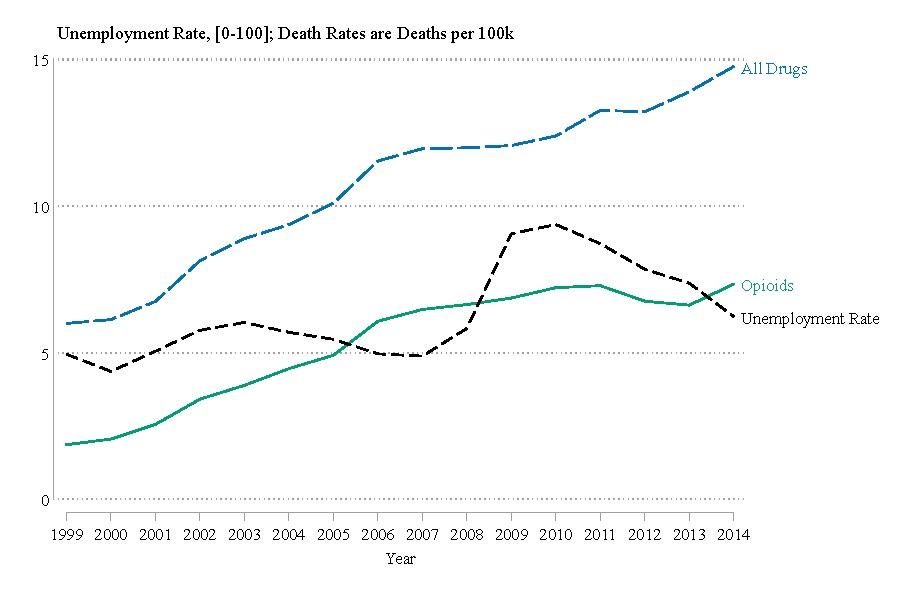
\includegraphics[width=\linewidth]{../results/figures/figure_1_death_rates_over_time.pdf}
		\end{center}		
		\label{fig:death_by_type_and_unemployment}
	 	\footnotesize{\subcaption*{\emph{Source:} Author calculations using National Vital Statistics System of the Centers for Disease Control and Prevention Multiple Cause of Death (MCOD) files for 1999-2014, together with unemployment rates from the Bureau of Labor Statistics.}}	
\end{figure}

%------------------------------------------%
%			Figure 2
% Drug Deaths by Race
%------------------------------------------%
\begin{figure}[ht!]
		\centering
		\caption{Total Opioid Death Rate by Race, 1999-2014}
\begin{center}
			  	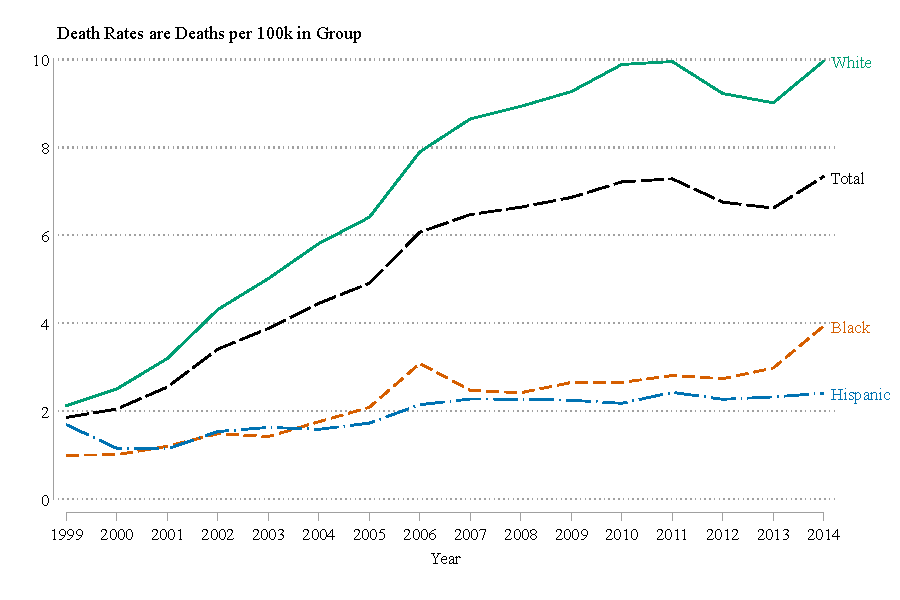
\includegraphics[width=\linewidth]{../results/figures/figure_2_opioid_deaths_by_race_over_time.pdf}
		\end{center}		\label{fig:opioid_deaths_by_race_and_time}
	 	\footnotesize{\subcaption*{\emph{Source:} Author calculations using National Vital Statistics System of the Centers for Disease Control and Prevention Multiple Cause of Death (MCOD) files for 1999-2014.}}
\end{figure}

%------------------------------------------%
%			Figure 3
% Figure of ED Visits by State by Type for Overdoses 
%------------------------------------------%
\begin{figure}[ht!]
\centering
		\caption{Opioid and All Drug Overdose ED Visit Rate, 2006-2014}
\begin{center}
			  	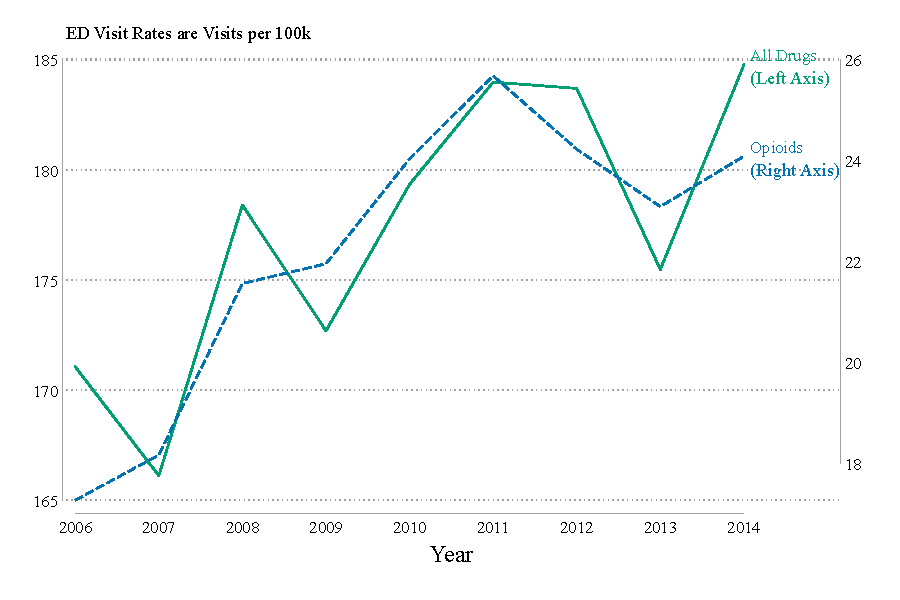
\includegraphics[width=\linewidth]{../results/figures/figure_3_drug_op_ed_rate_06_14.pdf}
		\end{center}		\label{fig:drug_opioid_deaths_by_race_and_time}
  		\label{fig:ed_by_type}
	 	\footnotesize{\subcaption*{\emph{Source:} Author calculations using the Healthcare Cost and Utilization Project's Nationwide Emergency Department Sample for 2006-2014.}}
\end{figure}

%------------------------------------------%
%			Figure 4
% Drug Overdose ED Visit Rate by Major Drug Type
%------------------------------------------%
\begin{figure}[ht!]
		\centering
		\caption{Drug Overdose ED Visit Rate by Major Drug Type, 2006-2014}
\begin{center}
			  	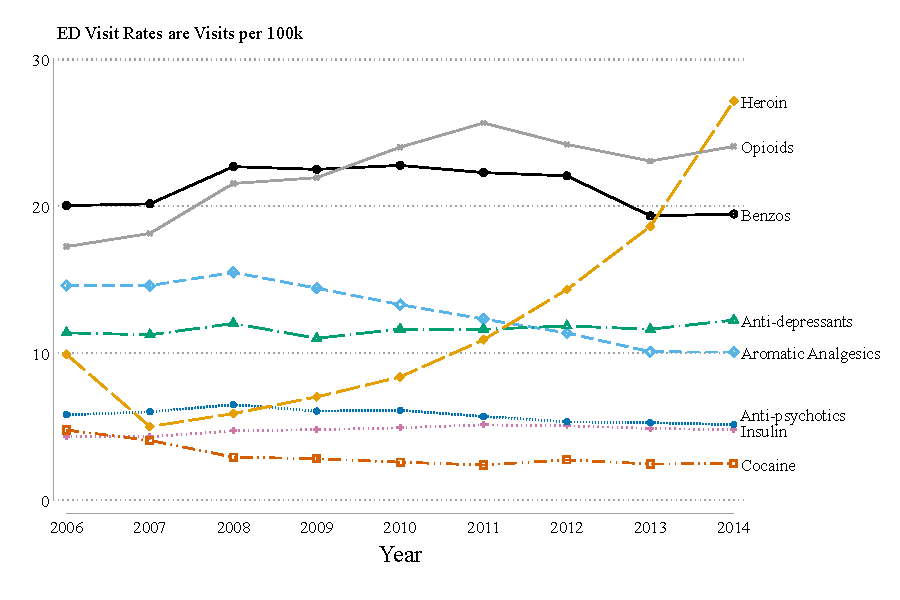
\includegraphics[width=\linewidth]{../results/figures/figure_4_top_drug_ed_rate_06_14.pdf}
		\end{center}		\label{fig:ed_visits_by_drug_by_time}
	 	\footnotesize{\subcaption*{\emph{Source:} Author calculations using the Healthcare Cost and Utilization Project's Nationwide Emergency Department Sample for 2006-2014.}	}
\end{figure}

%%%%%%%%%%%%%%%%%%%%%%%%%%%%%%%%%%%%%%%%%%%%%%%%%%%%%
%%%%%%%%%%%%%%%%%%%%%%%%%%%%%%%%%%%%%%%%%%%%%%%%%%%%%
%------------------------------------------%
%			Tables
%------------------------------------------%
%%%%%%%%%%%%%%%%%%%%%%%%%%%%%%%%%%%%%%%%%%%%%%%%%%%%%
%%%%%%%%%%%%%%%%%%%%%%%%%%%%%%%%%%%%%%%%%%%%%%%%%%%%%
%------------------------------------------%
%			Table 1: Data explanation
%------------------------------------------%
\begin{table}[]
\centering
\caption{Emergency Department Data: Geographic Detail and Years Used in Analysis}
\label{my-label}
\begin{tabular}{@{}ccccc@{}}
\toprule
State          & County-Level Data & County-Level Years           & State-Level Data & State-Level Years           \\ \midrule
Arizona        & Yes               & 2005-2014       & Yes              & 2005-2013       \\
Florida        & Yes               & 2005-2014       & Yes              & 2005-2013       \\
Hawaii         & No                &                 & Yes              & 2003-2010, 2013 \\
Iowa           & No                &                 & Yes              & 2004-2013       \\
Illinois       & No                &                 & Yes              & 2009-2013       \\
Kentucky       & Yes               & 2008-2012       & Yes              & 2008-2013       \\
Maryland       & Yes               & 2002-2012       & Yes              & 2005-2013       \\
Minnesota      & No                &                 & Yes              & 2001-2013       \\
North Carolina & No                &                 & Yes              & 2007-2013       \\
Nebraska       & No                &                 & Yes              & 2001-2011, 2013 \\
New Hampshire  & No                &                 & Yes              & 2003-2009       \\
New Jersey     & Yes               & 2004, 2006-2013 & No               &                 \\
South Carolina & No                &                 & Yes              & 2005-2013       \\
Tennessee      & No                &                 & Yes              & 2005-2013       \\
Utah           & No                &                 & Yes              & 2000-2013       \\
Vermont        & No                &                 & Yes              & 2002-2013       \\ \bottomrule
\end{tabular}
\Fignote{\footnotesize{County-level data are constructed from the micro-data (visit-level) provided by the Healthcare Cost and Utilization Project's (HCUP) State Emergency Department Databases (SEDD). The state-level data is taken directly from the ``State Statistics on All ED Visits'' portion of HCUPNet, available at \href{https://hcupnet-archive.ahrq.gov}{https://hcupnet-archive.ahrq.gov}.}}
\end{table}
\newpage

%------------------------------------------%
%	Table 2: Summary Statistics Table
%------------------------------------------%
	\begin{table}[ht!]\centering
			\begin{adjustbox}{width=\textwidth}
			\centering
			  \begin{threeparttable}
			    \caption[Summary Statistics]{County-Level Summary Statistics for Drug Related Deaths and ED Visits}
			    \estauto{../results/tables/table_2_summary_statistics_weighted}{8}{S[table-format=1.2,table-column-width=17mm]}
			    \label{tab:summary_statistics_weighted_main}
			   % \Figtext{Some basic text about the table.}
			    %\Fignote{These summary data are county-year and state-year. }
			    \Figsource{Mortality data are at the county-year and come from the Centers for Disease Control and Prevention's Multiple Cause of Death files from 1999-2014 and are adjusted as in text. ED data at the county-year level and are provided via the Healthcare Cost and Utilization Project's State Emergency Department Databases (SEDD). SEDD data come from Arizona (2005-2014), Kentucky (2008, 2010-2012), Florida (2005-2014), Maryland (2002-2012), and New Jersey (2004, 2006-2103). See text for ICD-9 definitions of outcomes. County level unemployment data come from Bureau for Labor Statistics. Unemployment rate, death rates, and ED visit rates are all weighted by total county population of group. Hispanic ED visits are omitted as the ED data do not contain a reliable indicator of Hispanic ethnicity.}
			  %  \Starnote
			  \end{threeparttable}
			 \end{adjustbox}
		\end{table}

%------------------------------------------%
% Table 3: County-level estimates by model
%------------------------------------------%
\newpage
	\begin{table}[ht]\centering
			\begin{adjustbox}{width=.75\textwidth}
			\centering
			  \begin{threeparttable}
			    \caption[County-Level Specifications, All Races Combined]{The estimated effect of county-level unemployment on the rate of opioid/drug mortality and emergency department visits across multiple specifications.}
			    \estauto{../results/tables/table_3_all_county_combined_robust_se}{5}{S[table-format=1.2,table-column-width=17mm]}
			    \label{tab:county_level_all_specs}
			   % \Figtext{Some basic text about the table.}
				\small{\Fignote{* p $<$ 0.1, ** p $<$ 0.05, *** p $<$ 0.01. Robust standard errors clustered at the county level in parentheses. Each regression is weighted by total county population.}} 
			  % \Starnote
			  \end{threeparttable}
			 \end{adjustbox}
		\end{table}

%------------------------------------------%
% Table 4: Perferred Specification by Race
%------------------------------------------%
	\begin{table}[ht]\centering
			\begin{adjustbox}{width=.8\textwidth}
			\centering
			  \begin{threeparttable}
			    \caption[County-Level Preferred Specification by Race]{The estimated effect of county-level unemployment on the rate of opioid/drug mortality and emergency department visits for our preferred specification across race/ethnicity.}
			    \estauto{../results/tables/table_4_county_by_race}{9}{S[table-format=1.2,table-column-width=17mm]}
			    \label{tab:county_level_by_race_perferred_spec}
			   % \Figtext{Some basic text about the table.}
				\small{\Fignote{* p $<$ 0.1, ** p $<$ 0.05, *** p $<$ 0.01. Robust standard errors clustered at the county level in parentheses. All specifications include county fixed-effects, year fixed-effects, and state-by-year fixed effects. Each regression is weighted by county population of group. Hispanic ED visits are omitted as the ED data do not contain a reliable indicator of Hispanic ethnicity.} }
			  \end{threeparttable}
			 \end{adjustbox}
		\end{table}

%------------------------------------------%
% Table 5: State-level estimates
%------------------------------------------%
	\begin{table}[ht]\centering
			\begin{adjustbox}{width=\textwidth}
			\centering
			  \begin{threeparttable}
			    \caption[State-Level Specifications, All Races]{The estimated effect of state-level unemployment on the rate of opioid/drug mortality and emergency department visits across multiple specifications and race/ethnicity.}
			    \estauto{../results/tables/table_5_state_deaths_by_type}{9}{S[table-format=1.2,table-column-width=17mm]}
			    \label{tab:state_level_deaths}
			   % \Figtext{Some basic text about the table.}
			    \small{\Fignote{* p $<$ 0.1, ** p $<$ 0.05, *** p $<$ 0.01. Robust standard errors clustered at the state level in parentheses. Each regression is weighted by total state population of group. Hispanic ED visits are omitted as the ED data do not contain a reliable indicator of Hispanic ethnicity.}}
			    %\Figsource{We good the data from here.}
			    %\Starnote
			  \end{threeparttable}
			 \end{adjustbox}
		\end{table}

%%%%%%%%%%%%%%%%%%%%%%%%%%%%%%%%%%%%%%%%%%%%%%%%%%%%%
%%%%%%%%%%%%%%%%%%%%%%%%%%%%%%%%%%%%%%%%%%%%%%%%%%%%%
%------------------------------------------%
%			Appendix
%------------------------------------------%
%%%%%%%%%%%%%%%%%%%%%%%%%%%%%%%%%%%%%%%%%%%%%%%%%%%%%
%%%%%%%%%%%%%%%%%%%%%%%%%%%%%%%%%%%%%%%%%%%%%%%%%%%%%
\appendix
\setcounter{table}{0}
\renewcommand{\thetable}{A\arabic{table}}
\setcounter{figure}{0}
\renewcommand{\thefigure}{A\arabic{figure}}

\FloatBarrier
%%%%%%%%%%%%%%%%%%%%%%%%%%%%%%%%%%%%%%%%%%%%%%%%%%%%%
%%%%%%%%%%%%%%%%%%%%%%%%%%%%%%%%%%%%%%%%%%%%%%%%%%%%%
%------------------------------------------%
%			Appendix Figures
%------------------------------------------%
%%%%%%%%%%%%%%%%%%%%%%%%%%%%%%%%%%%%%%%%%%%%%%%%%%%%%
%%%%%%%%%%%%%%%%%%%%%%%%%%%%%%%%%%%%%%%%%%%%%%%%%%%%%
%------------------------------------------%
%			Figure A1
%Limit Years
%------------------------------------------%
\begin{figure}[h]
	\caption[Excluding three year bins]{The estimated effect of county-level unemployment on the rate of opioid/drug mortality and emergency department visits excluding various three-year bins.}
	\begin{minipage}[c]{0.48\linewidth}
		\centering
		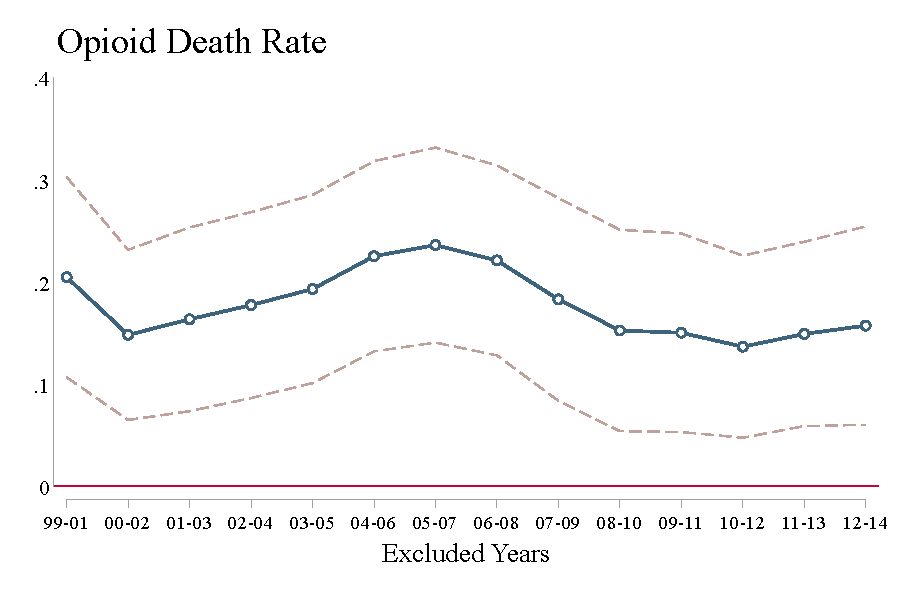
\includegraphics[width=\linewidth]{../results/appendix/figures/aopioidr_drop_years.pdf}
	  	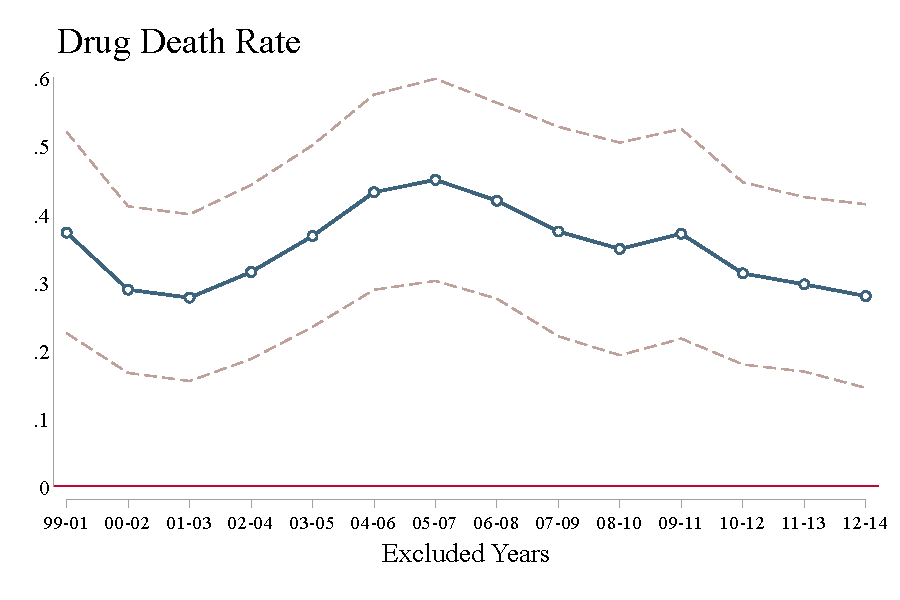
\includegraphics[width=\linewidth]{../results/appendix/figures/drugr_drop_years.pdf}
	\end{minipage}
	~
	\hspace{0.05cm}
	\begin{minipage}[c]{0.48\linewidth}\centering
	  \centering
	  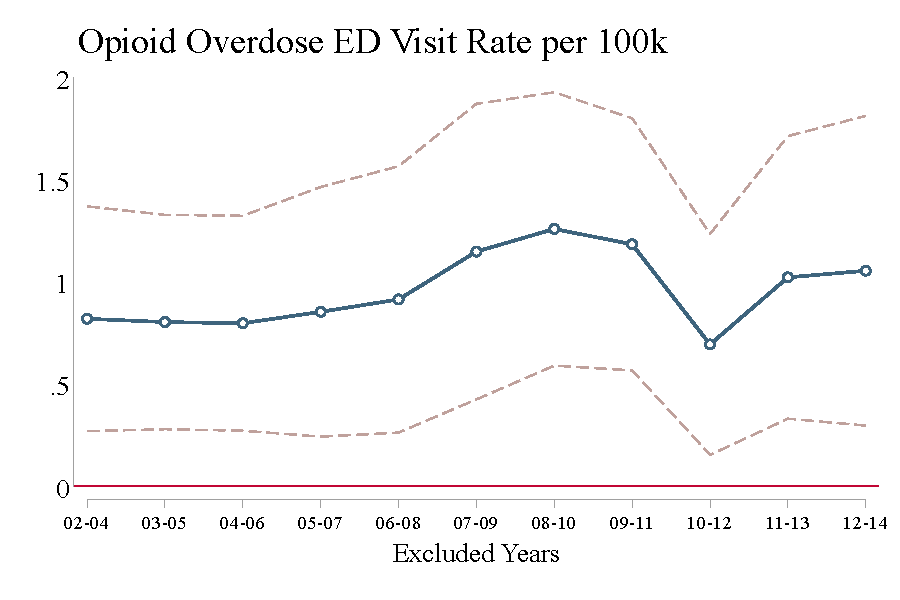
\includegraphics[width=\linewidth]{../results/appendix/figures/r_op_ovr_total_drop_years.pdf}
	 	  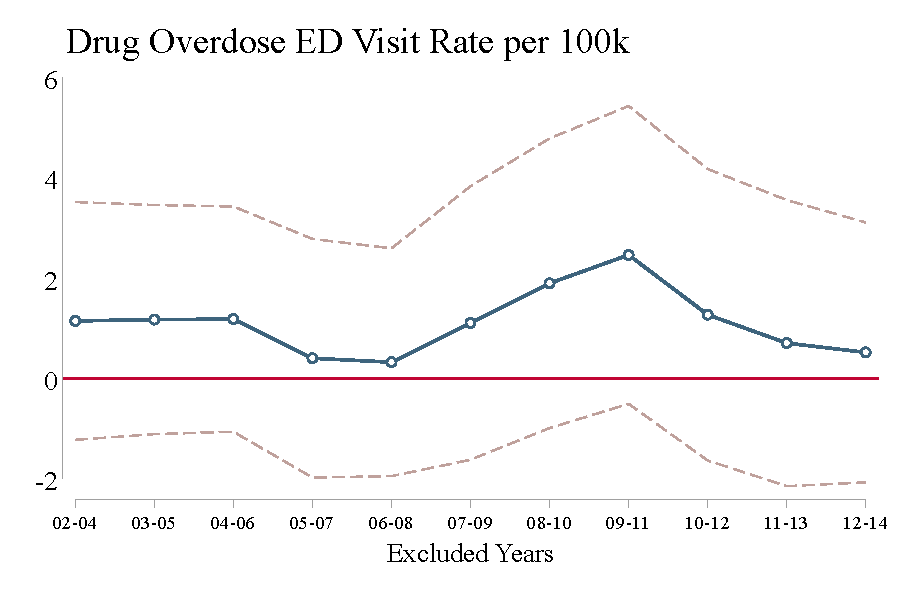
\includegraphics[width=\linewidth]{../results/appendix/figures/r_drug_ovr_total_drop_years.pdf}
	\end{minipage}
	 	\subcaption*{\emph{Note:} Each point is from a separate regression that corresponds to our preferred specification in the text. Each regression has county fixed-effects, year fixed-effects,  and state-by-year fixed effects. Each regression excludes the years noted. 95\% confidence intervals are displayed by dashed lines and are calculated using robust standard errors clustered at the county level. Each regression is weighted by total county population.}	
	\label{fig:limit_years}
\end{figure}

\FloatBarrier
%------------------------------------------%
%			Figure A2
	%Population Density 
%------------------------------------------%
			\newpage
		\FloatBarrier
		\begin{figure}[h]
			\caption[Excluding population density quintiles]{The estimated effect of county-level unemployment on the rate of opioid/drug mortality and emergency department visits excluding population density quintiles.}
			\begin{minipage}[c]{0.48\linewidth}
				\centering
				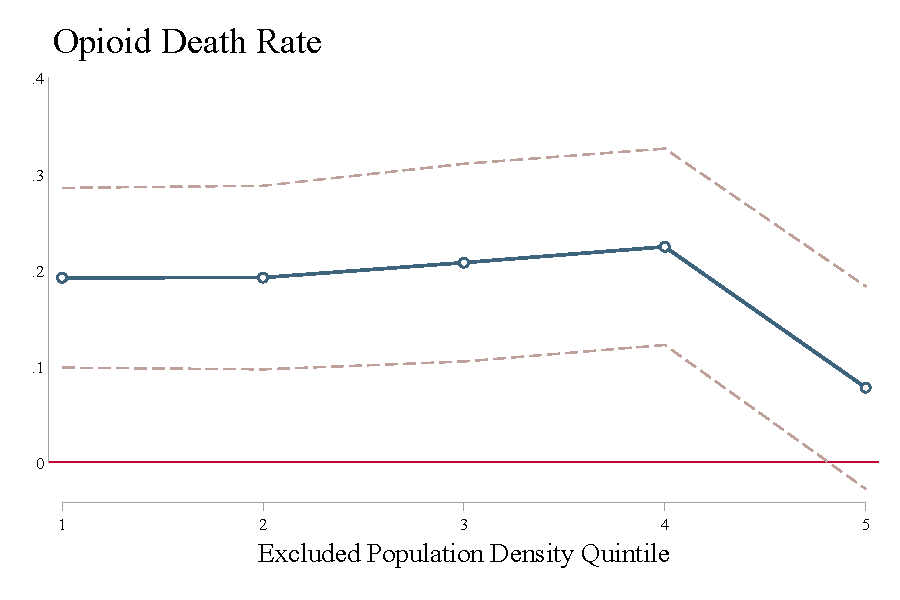
\includegraphics[width=\linewidth]{../results/appendix/figures/opioid_by_pop_den_quintile.pdf}
							  	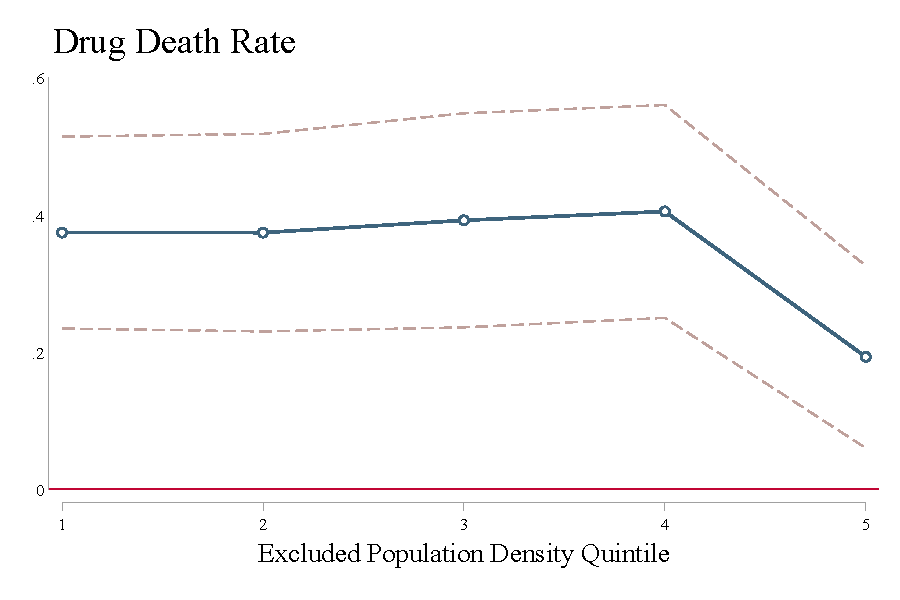
\includegraphics[width=\linewidth]{../results/appendix/figures/drug_by_pop_den_quintile.pdf}
			\end{minipage}
			~
			\hspace{0.05cm}
			\begin{minipage}[c]{0.48\linewidth}\centering
			  \centering
			  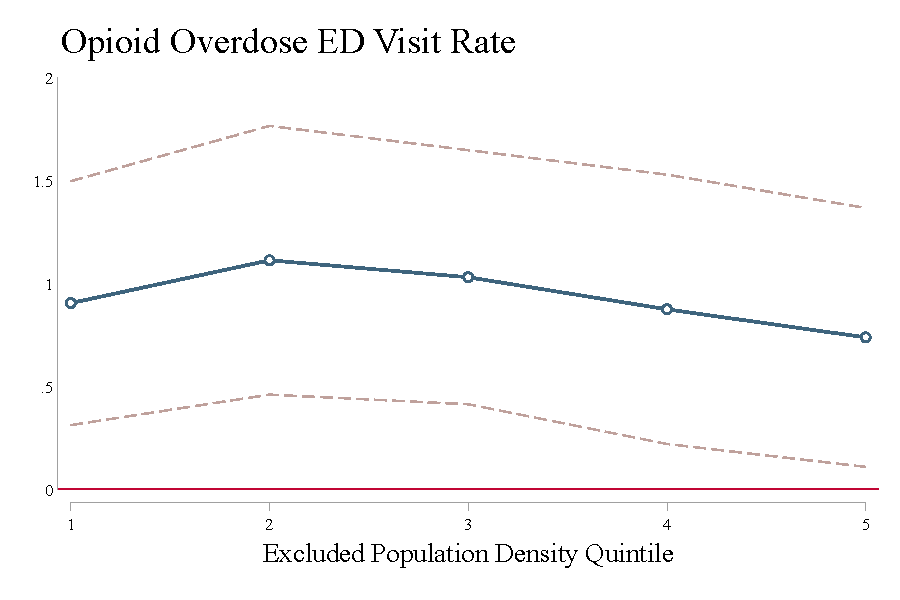
\includegraphics[width=\linewidth]{../results/appendix/figures/op_ovr_by_pop_den_quintile.pdf}			
			    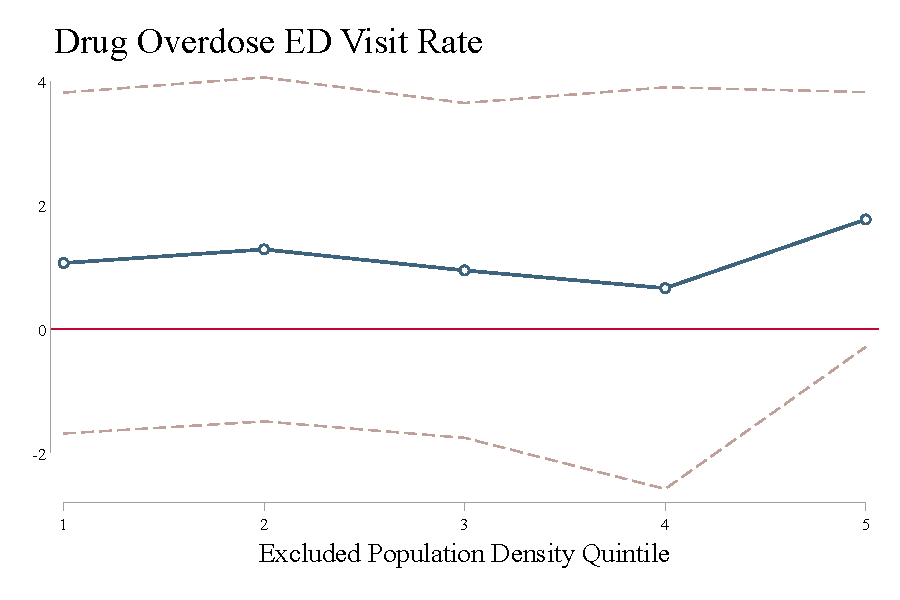
\includegraphics[width=\linewidth]{../results/appendix/figures/drug_ovr_by_pop_den_quintile.pdf}
			\end{minipage}
			\label{fig:pop_den}
	 	\subcaption*{\emph{Note:} Each point is from a separate regression that corresponds to our preferred specification in the text. Each regression has county fixed-effects, year fixed-effects, and state-by-year fixed effects.  Each regression excludes the quintile noted. 95\% confidence intervals are displayed by dashed lines and are calculated using robust standard errors clustered at the county level. Each regression is weighted by total county population.}	
		\end{figure}

%------------------------------------------%
%			Figure A3
	%High School Graduation  
%------------------------------------------%
		\newpage
		\FloatBarrier
		\begin{figure}[h]
			\begin{minipage}[c]{0.48\linewidth}
				\centering
				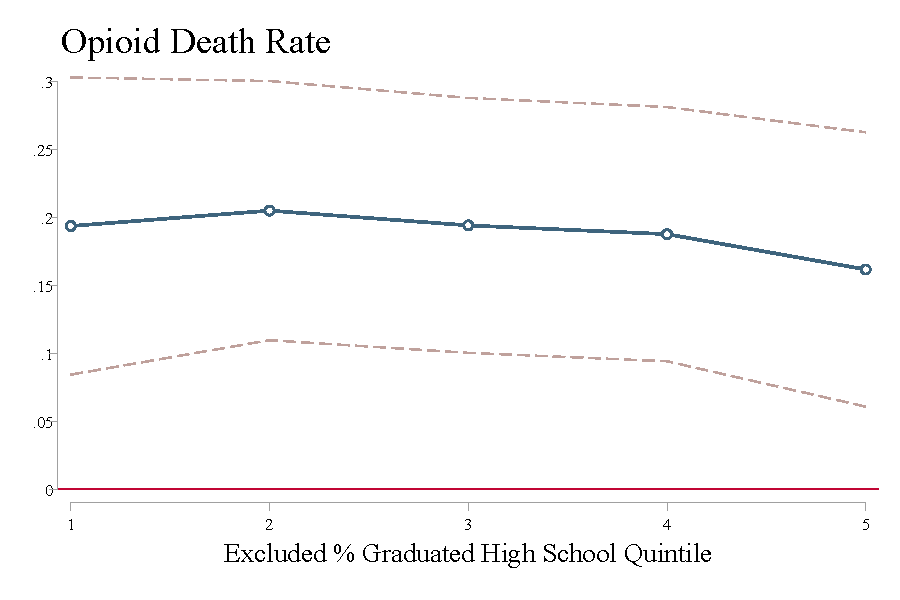
\includegraphics[width=\linewidth]{../results/appendix/figures/opioid_by_hs_quintile.pdf}
			  	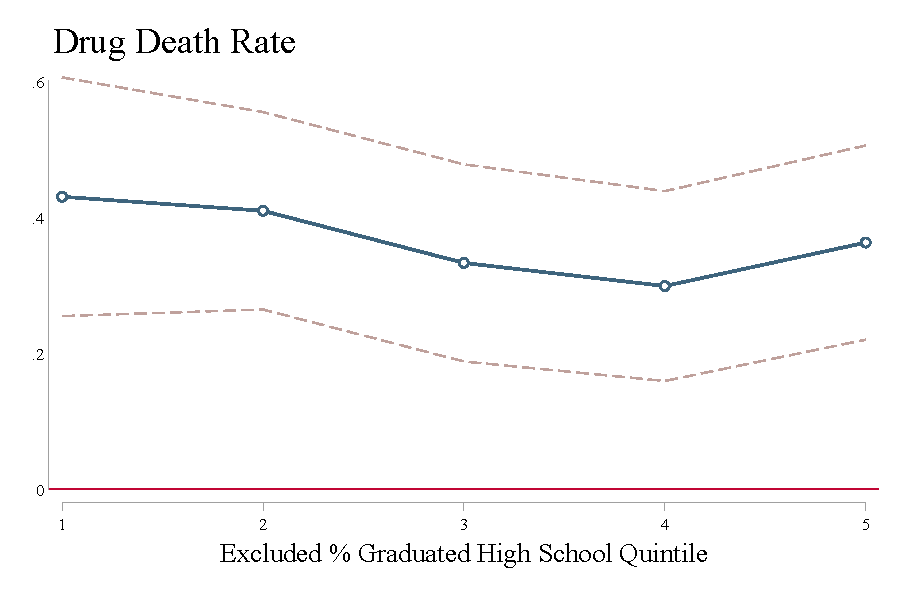
\includegraphics[width=\linewidth]{../results/appendix/figures/drug_by_hs_quintile.pdf}
			\end{minipage}
			~
			\hspace{0.05cm}
			\begin{minipage}[c]{0.48\linewidth}\centering
			  \centering
			  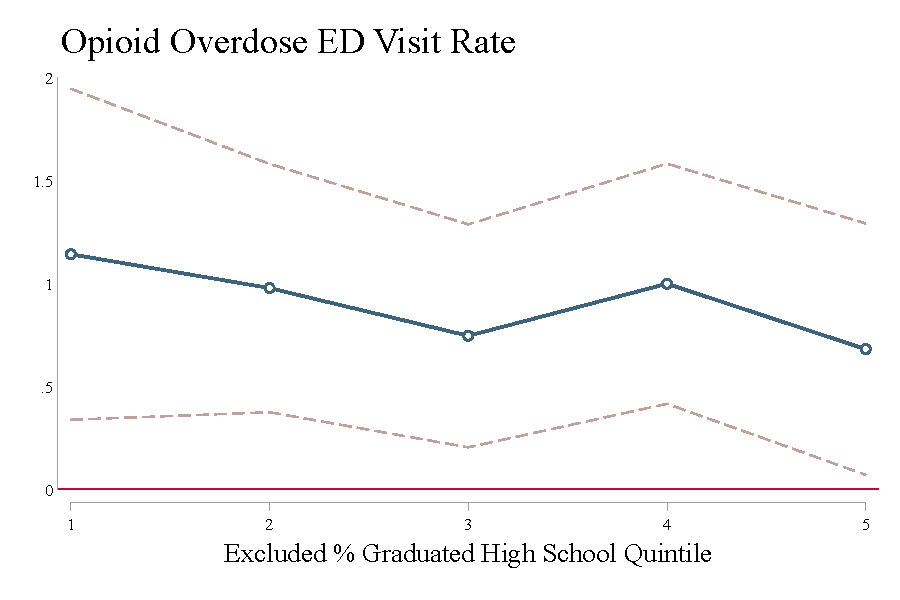
\includegraphics[width=\linewidth]{../results/appendix/figures/op_ovr_by_hs_quintile.pdf}
			  			  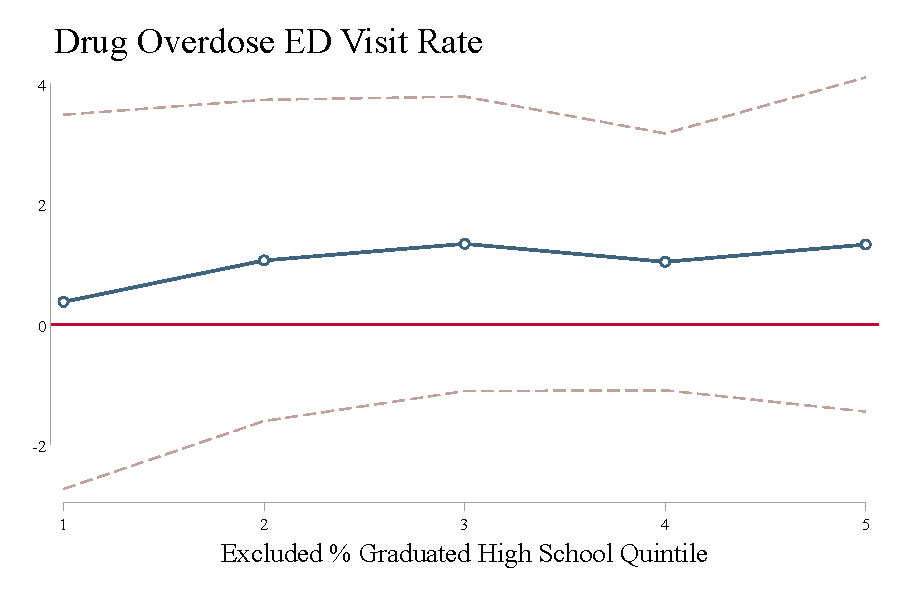
\includegraphics[width=\linewidth]{../results/appendix/figures/drug_ovr_by_hs_quintile.pdf}
			\end{minipage}
			\caption[Excluding \% graduated high school quintiles]{The estimated effect of county-level unemployment on the rate of opioid/drug mortality and emergency department visits excluding \% graduated high school quintiles}
			\label{fig:high_school}
	 	\subcaption*{\emph{Note:} Each point is from a separate regression that corresponds to our preferred specification in the text. Each regression has county fixed-effects, year fixed-effects, and state-by-year fixed effects.  Each regression excludes the quintile noted. 95\% confidence intervals are displayed by dashed lines and are calculated using robust standard errors clustered at the county level. Each regression is weighted by total county population.}	
		\end{figure}

%------------------------------------------%
%			Figure A4
	%Percent Non-White
%------------------------------------------%
		\newpage
		\FloatBarrier
		\begin{figure}[h]
			\begin{minipage}[c]{0.48\linewidth}
				\centering
								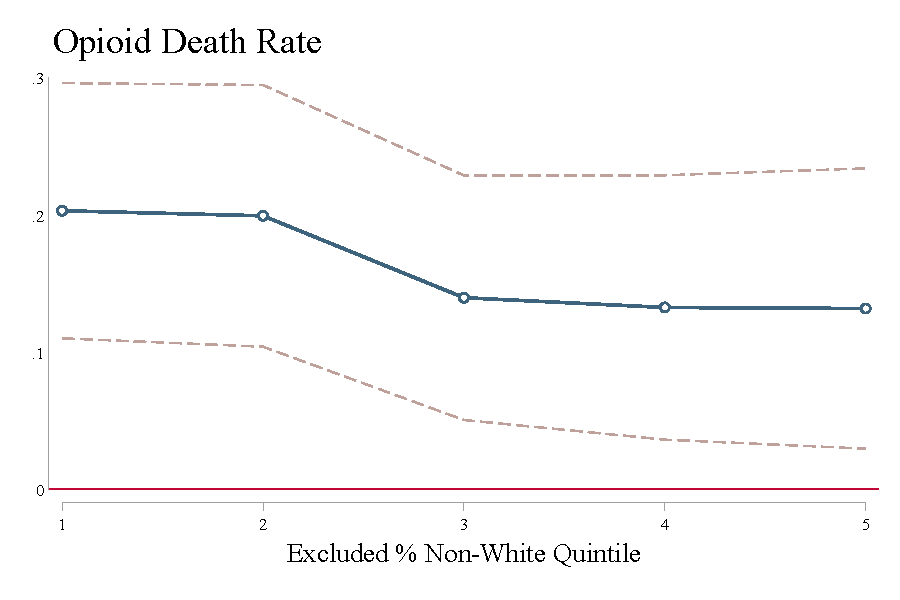
\includegraphics[width=\linewidth]{../results/appendix/figures/opioid_by_pnw_quintile.pdf}
			  	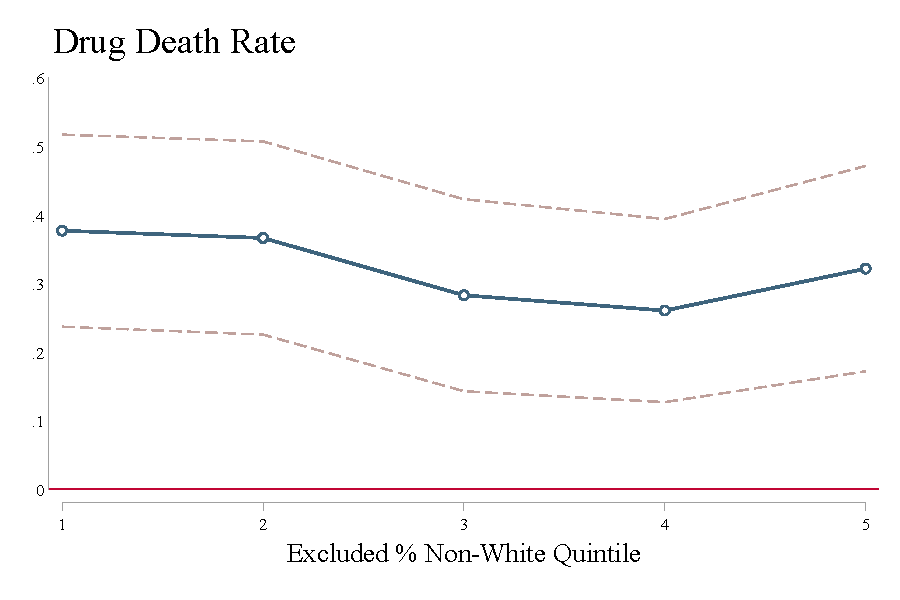
\includegraphics[width=\linewidth]{../results/appendix/figures/drug_by_pnw_quintile.pdf}
			\end{minipage}
			~
			\hspace{0.05cm}
			\begin{minipage}[c]{0.48\linewidth}\centering
			  \centering
			  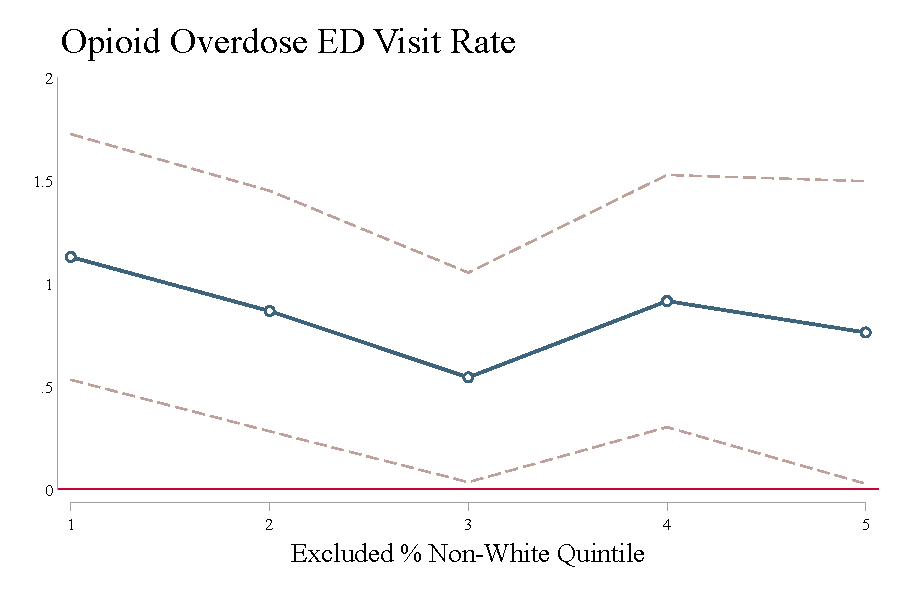
\includegraphics[width=\linewidth]{../results/appendix/figures/op_ovr_by_pnw_quintile.pdf}
			  					  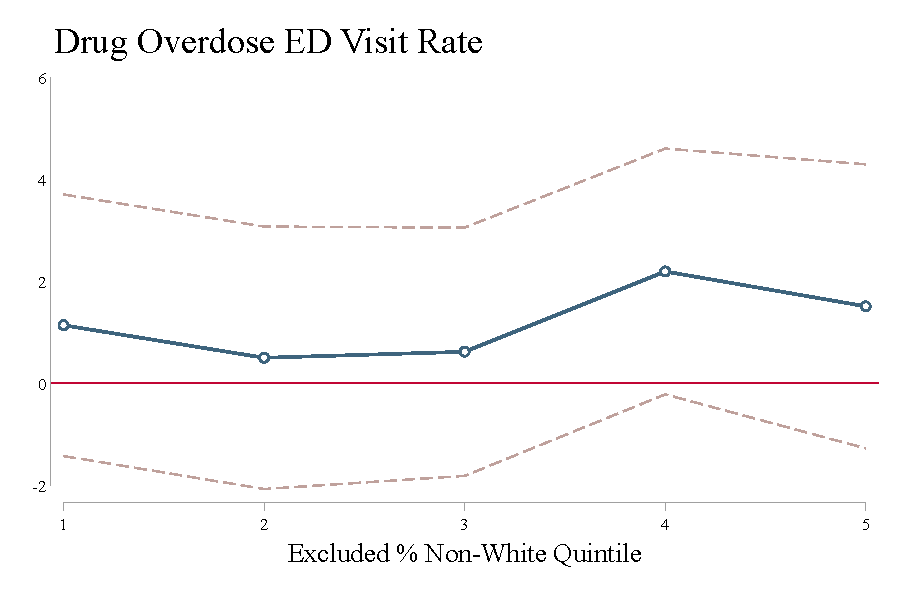
\includegraphics[width=\linewidth]{../results/appendix/figures/drug_ovr_by_pnw_quintile.pdf}
			\end{minipage}
			\caption[Excluding \% non-white quintiles]{The estimated effect of county-level unemployment on the rate of opioid/drug mortality and emergency department visits excluding \% non-white quintiles}
			\label{fig:percent_non_white}
	 	\subcaption*{\emph{Note:} Each point is from a separate regression that corresponds to our preferred specification in the text. Each regression has county fixed-effects, year fixed-effects, and state-by-year fixed effects.  Each regression excludes the quintile noted. 95\% confidence intervals are displayed by dashed lines and are calculated using robust standard errors clustered at the county level. Each regression is weighted by total county population.}	
		\end{figure}

%------------------------------------------%
%			Figure A5
%Change in % Manufacturing Employment  
%------------------------------------------%
		\newpage
		\FloatBarrier
		\begin{figure}[h]
			\begin{minipage}[c]{0.48\linewidth}
				\centering
				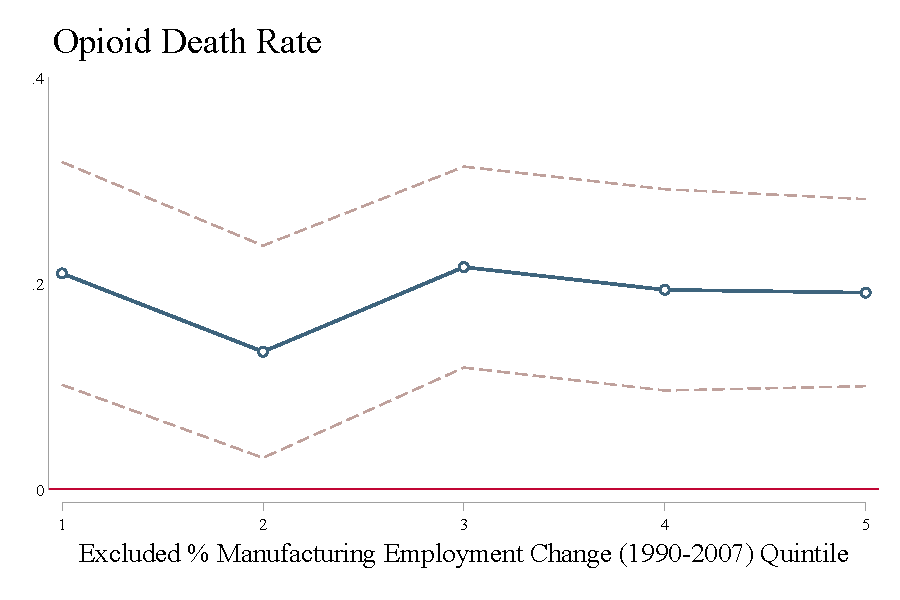
\includegraphics[width=\linewidth]{../results/appendix/figures/opioid_by_man_quintile.pdf}
						  	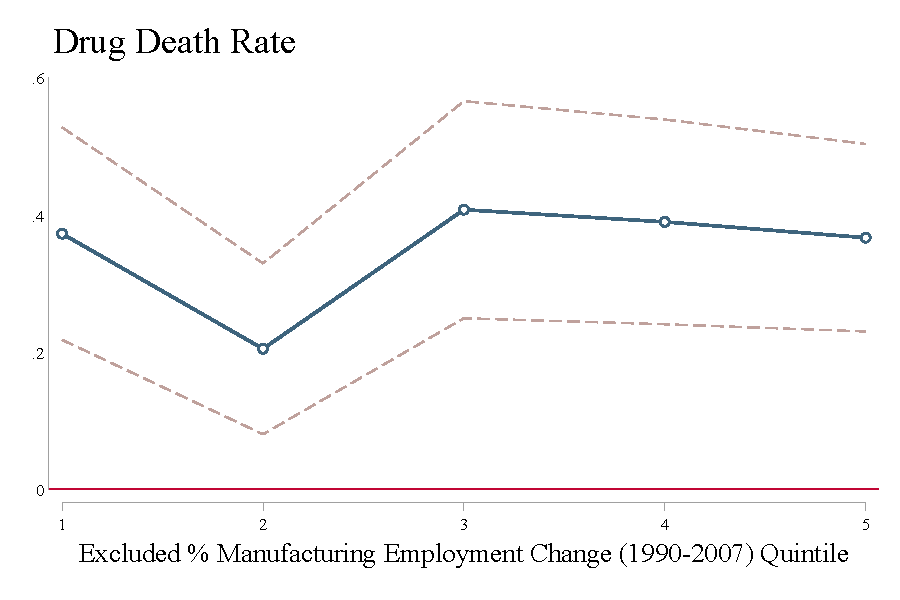
\includegraphics[width=\linewidth]{../results/appendix/figures/drug_by_man_quintile.pdf}
			\end{minipage}
			~
			\hspace{0.05cm}
			\begin{minipage}[c]{0.48\linewidth}\centering
			  \centering
			  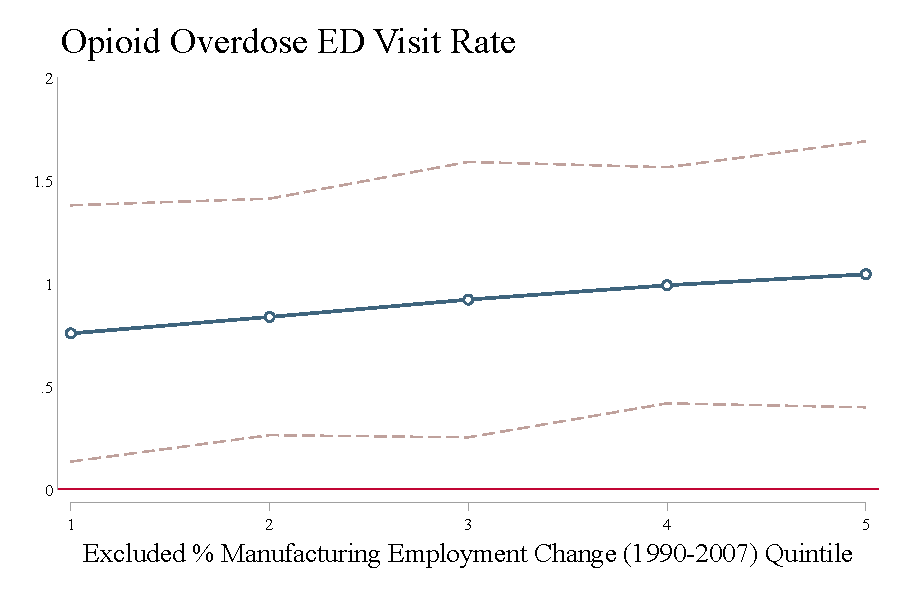
\includegraphics[width=\linewidth]{../results/appendix/figures/op_ovr_by_man_quintile.pdf}			  
			  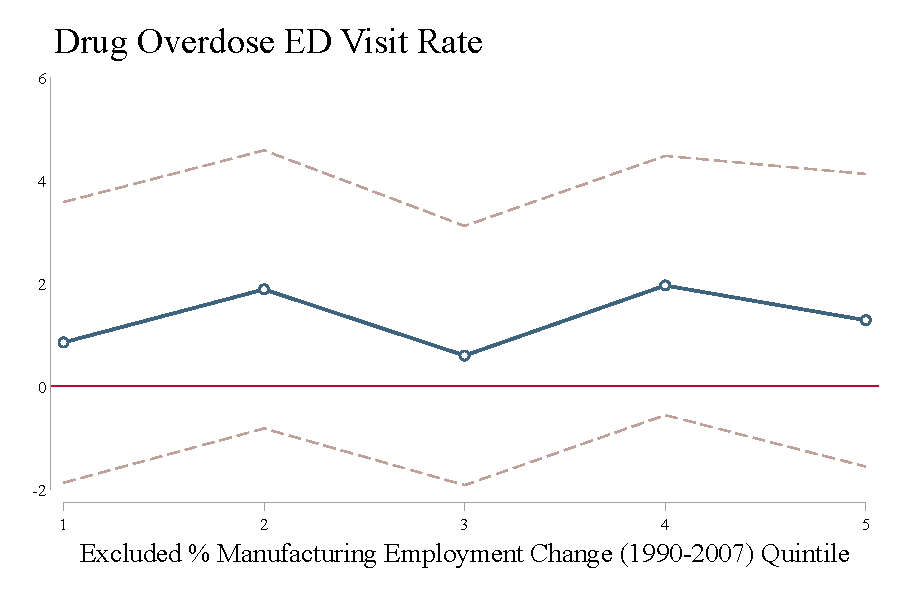
\includegraphics[width=\linewidth]{../results/appendix/figures/drug_ovr_by_man_quintile.pdf}
			\end{minipage}
			\caption[Excluding change in \% manufacturing employment (1990-2007) quintiles]{The estimated effect of county-level unemployment on the rate of opioid/drug mortality and emergency department visits excluding  change in \% manufacturing employment (1990-2007) quintiles}
			\label{fig:man}
				 	\subcaption*{\emph{Note:} Each point is from a separate regression that corresponds to our preferred specification in the text. Each regression has county fixed-effects, year fixed-effects, and state-by-year fixed effects.  Each regression excludes the quintile noted. 95\% confidence intervals are displayed by dashed lines and are calculated using robust standard errors clustered at the county level. Each regression is weighted by total county population. Data on change in manufacturing employment come from Autor et al. (2013). The lower the quintile, the larger the decrease in the share of manufacturing employment.}	
		\end{figure}

%------------------------------------------%
%			Figure A6
	%Change in Import Exposure
%------------------------------------------%	
		\newpage
		\FloatBarrier
		\begin{figure}[h]
			\begin{minipage}[c]{0.48\linewidth}
				\centering
			  	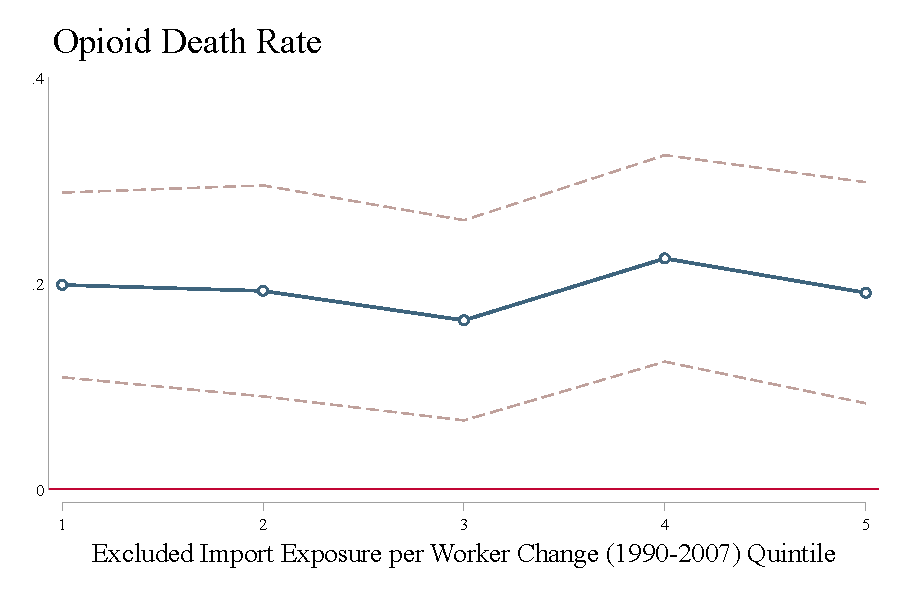
\includegraphics[width=\linewidth]{../results/appendix/figures/opioid_by_imp_exp_quintile.pdf}
				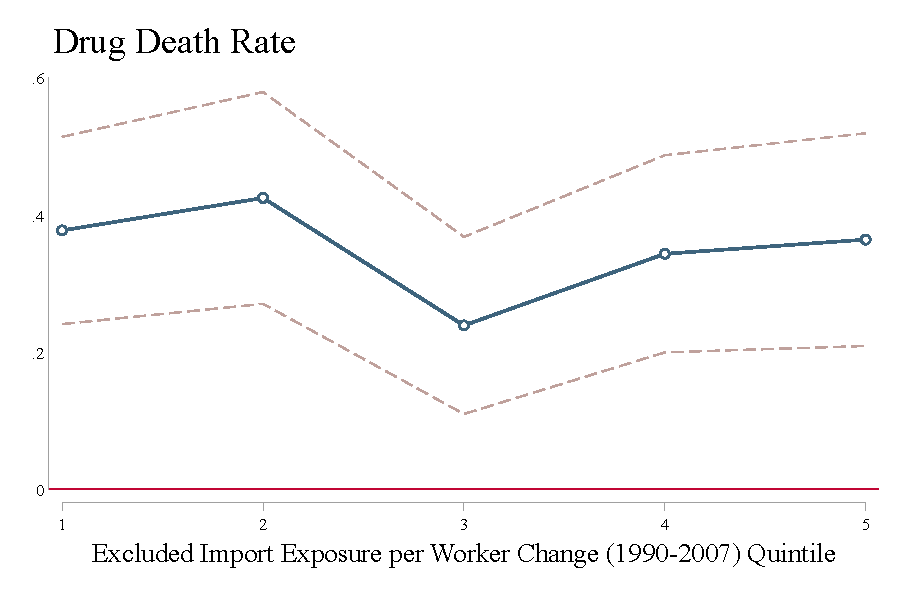
\includegraphics[width=\linewidth]{../results/appendix/figures/drug_by_imp_exp_quintile.pdf}
			\end{minipage}
			~
			\hspace{0.05cm}
			\begin{minipage}[c]{0.48\linewidth}\centering
			  \centering
			 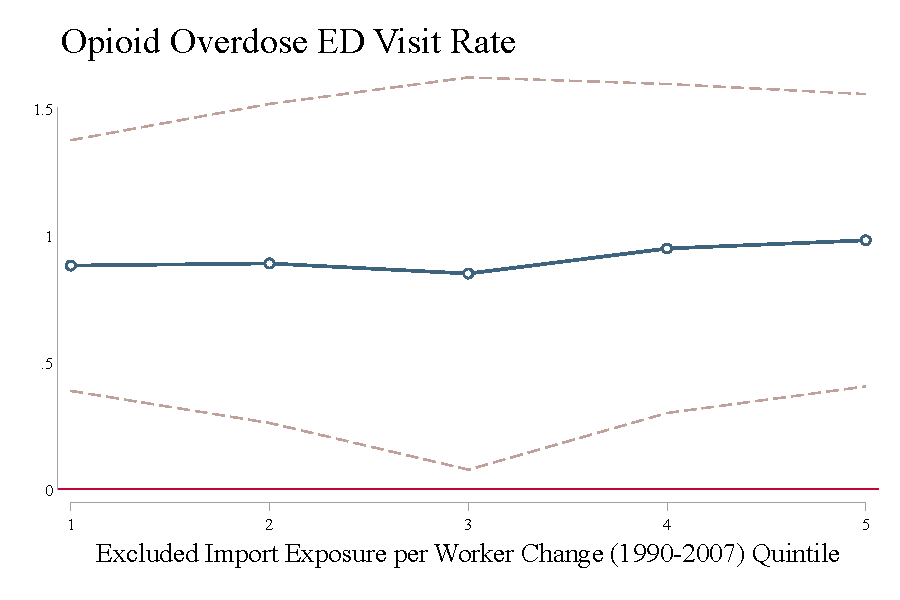
\includegraphics[width=\linewidth]{../results/appendix/figures/op_ovr_by_imp_exp_quintile.pdf}
			  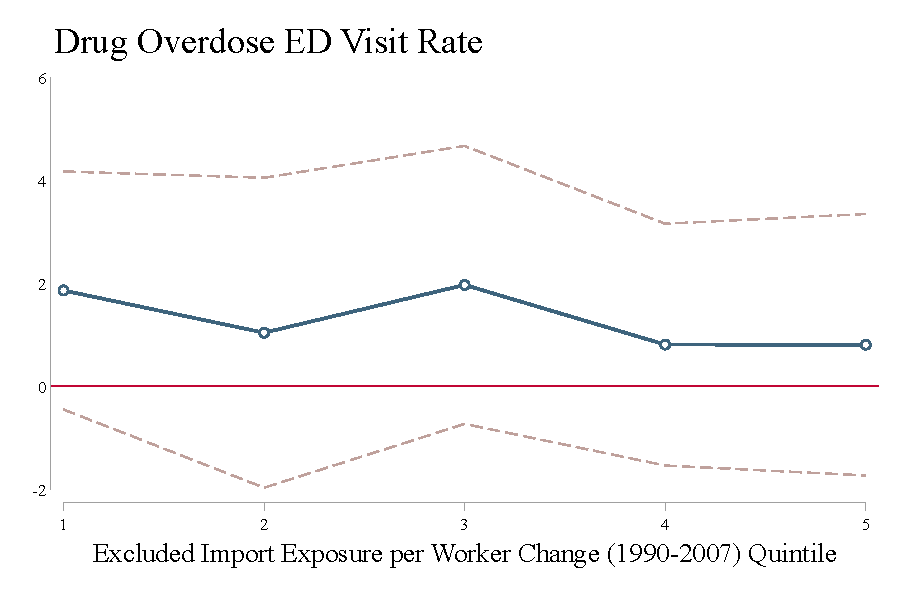
\includegraphics[width=\linewidth]{../results/appendix/figures/drug_ovr_by_imp_exp_quintile.pdf}
			\end{minipage}
			\caption[Excluding change in import exposure (1990-2007) quintiles]{The estimated effect of county-level unemployment on the rate of opioid/drug mortality and emergency department visits excluding  change in import exposure (1990-2007) quintiles}
			\label{fig:imp_exp}
				 	\subcaption*{\emph{Note:} Each point is from a separate regression that corresponds to our preferred specification in the text. Each regression has county fixed-effects, year fixed-effects, and state-by-year fixed effects.  Each regression excludes the quintile noted. 95\% confidence intervals are displayed by dashed lines and are calculated using robust standard errors clustered at the county level. Each regression is weighted by total county population. Data on change in manufacturing employment come from Autor et al. (2013). The lower the quintile, the smaller the change in import exposure.}	
		\end{figure}

%------------------------------------------%
%			Figure A7
%Placebos for ED Visits
%------------------------------------------%

		\newpage
		\FloatBarrier
		\begin{figure}[h]
				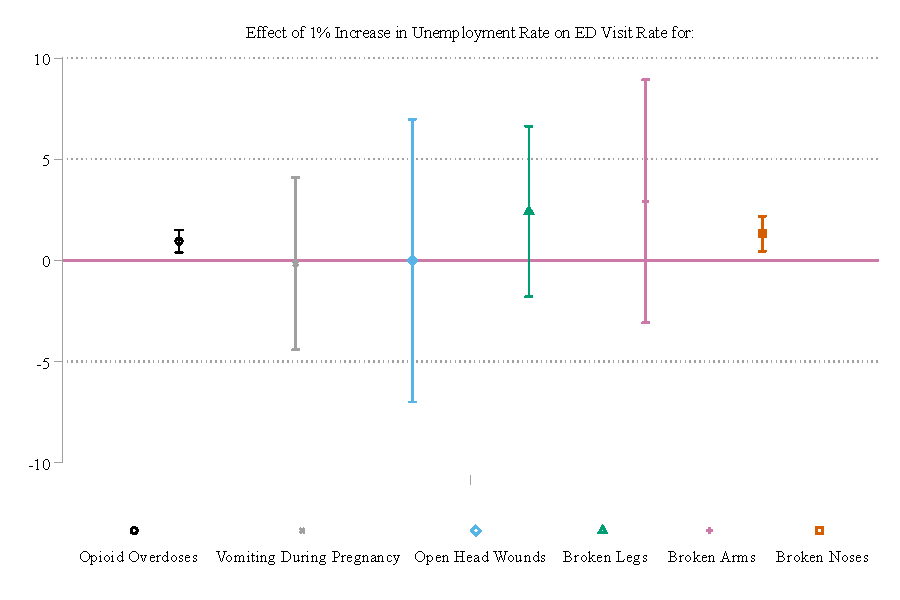
\includegraphics[width=\linewidth]{../results/appendix/figures/placebos.pdf}
			\caption[Placebo ED visits]{The effect of county-level unemployment on the rate of opioid ED visits and the rate of ED visits for various placebos.}
			\label{fig:placebos}
							 	\subcaption*{\emph{Note:} Each point is from a separate regression that corresponds to our preferred specification in the text. Each regression has county fixed-effects, year fixed-effects, and state-by-year fixed effects.  95\% confidence intervals are displayed by bracketed lines and are calculated using robust standard errors clustered at the county level. Each regression is weighted by total county population.}	
		\end{figure}

%------------------------------------------%
%			Figure A8
% Figure of Opioid ED Visit effect by age and expected payer
%------------------------------------------%
				\FloatBarrier
		\begin{figure}[h]
				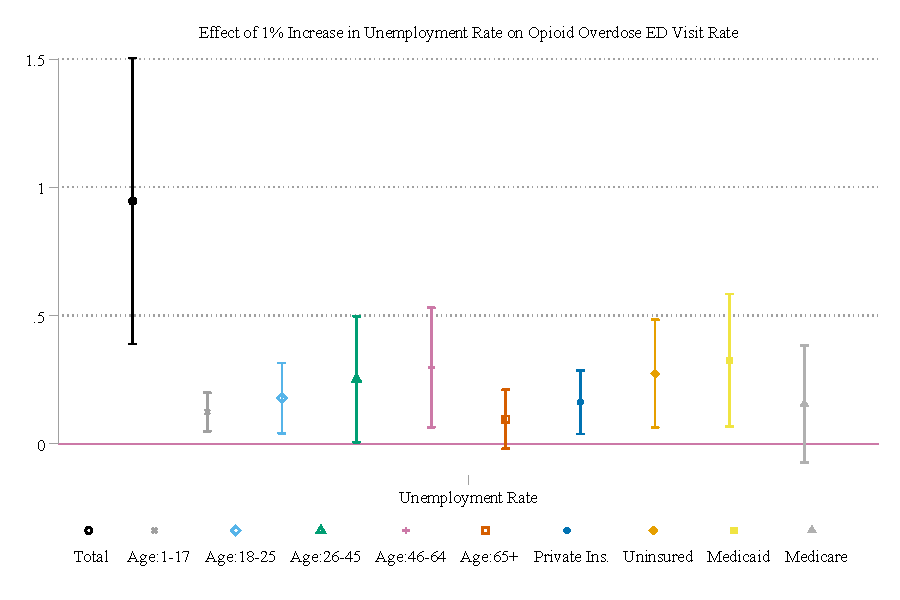
\includegraphics[width=\linewidth]{../results/appendix/figures/op_ovr_all_spec.pdf}
			\caption[Opioid ED visit rate by age and payer]{The effect of county-level unemployment on the opioid ED visit rate across various age groups and expected payer.}
			\label{fig:ovr_by_group}
							 	\subcaption*{\emph{Note:} Each point is from a separate regression that corresponds to our preferred specification in the text. Each regression has county fixed-effects, year fixed-effects, and state-by-year fixed effects.  95\% confidence intervals are displayed by bracketed lines and are calculated using robust standard errors clustered at the county level. Each regression is weighted by total county population.}	
			 \end{figure}
\FloatBarrier

%------------------------------------------%
%			Figure A9
	%All drug death rate by race and time
%------------------------------------------%
\begin{figure}[h]
		\centering
		\caption{All Drug Death Rate by Race, 1999-2014}
	  	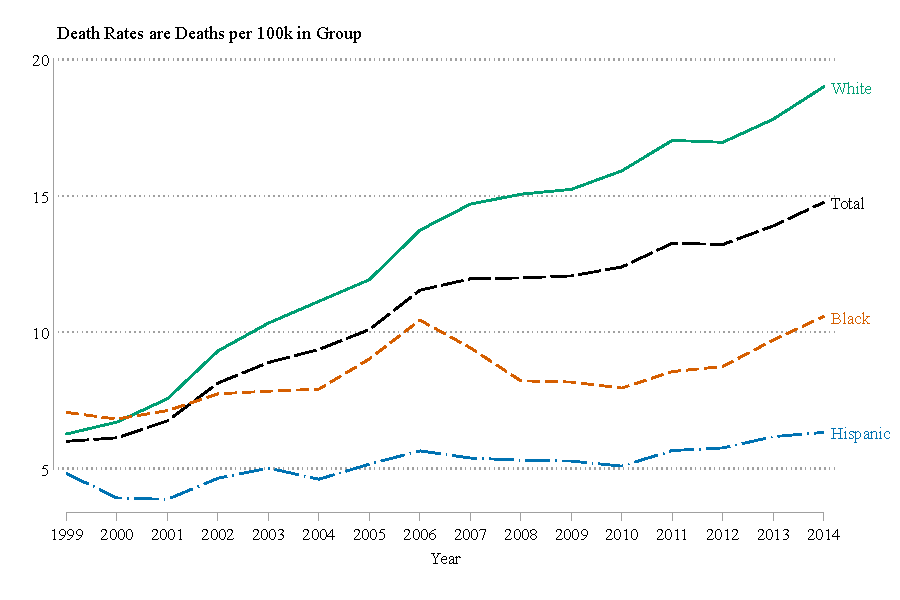
\includegraphics[width=\linewidth]{../results/appendix/figures/figure_A9_drug_deaths_by_race_over_time.pdf}
		\label{fig:drug_deaths_by_race_and_time}
\end{figure}

%------------------------------------------%
%			Figure A10
%			Power Analysis
%------------------------------------------%
	
\begin{figure}[h]
	\caption[Power Analysis for All Drug ED Visits]{Simulated Power Analysis For All Drug Overdose ED Visit Rate}
	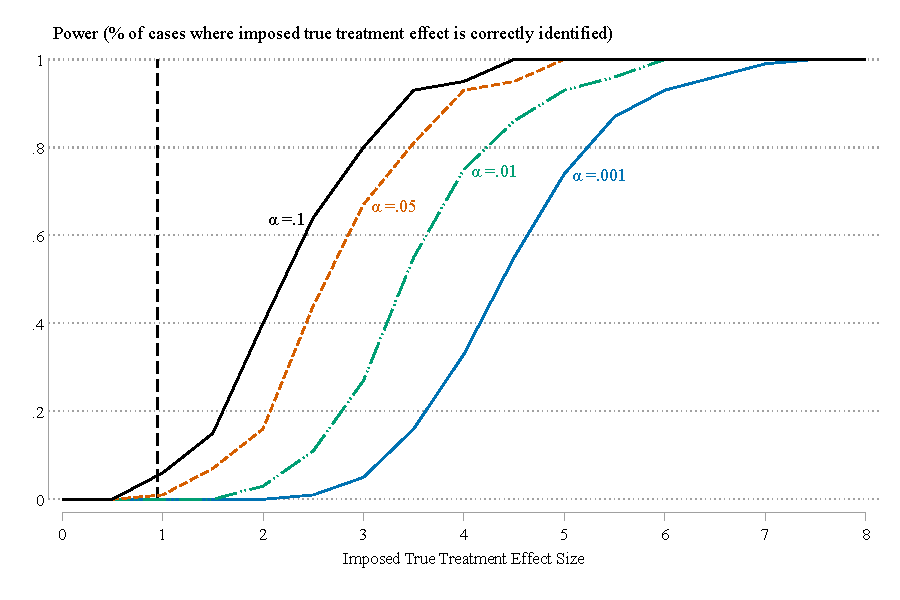
\includegraphics[width=\linewidth]{../results/appendix/figures/power_analysis_results.pdf}
	 \subcaption*{\emph{Note:} The dashed vertical line is the estimated effect size of 1 percentage point increase in the unemployment rate on the opioid overdose ED visit rate. $\alpha$ is the probability of a type I error.}	
	\label{fig:power_analysis}
\end{figure}


%%%%%%%%%%%%%%%%%%%%%%%%%%%%%%%%%%%%%%%%%%%%%%%%%%%%%
%%%%%%%%%%%%%%%%%%%%%%%%%%%%%%%%%%%%%%%%%%%%%%%%%%%%%
%------------------------------------------%
%			Appendix Tables
%------------------------------------------%
%%%%%%%%%%%%%%%%%%%%%%%%%%%%%%%%%%%%%%%%%%%%%%%%%%%%%
%%%%%%%%%%%%%%%%%%%%%%%%%%%%%%%%%%%%%%%%%%%%%%%%%%%%%

%------------------------------------------%
%			Table A1
% Different Time Trends
%------------------------------------------%
 		\begin{table}[ht]\centering
			\begin{adjustbox}{width=\textwidth}
			\centering
			  \begin{threeparttable}
			    \caption[Various types of time trends]{The estimated effect of county-level unemployment on the rate of opioid/drug mortality and emergency department visits across various types of time trends.}
			    \estauto{../results/appendix/tables/table_a1_different_time_trends}{7}{S[table-format=1.2,table-column-width=17mm]}
			    \label{tab:different_time_trends}
			   % \Figtext{Some basic text about the table.}
				\Fignote{* p $<$ 0.1, ** p $<$ 0.05, *** p $<$ 0.01. Robust standard errors clustered at the county level in parentheses. Each regression is weighted by total county population.}			    %\Figsource{We good the data from here.}
			  % \Starnote
			  \end{threeparttable}
			 \end{adjustbox}
		\end{table}

%------------------------------------------%
%			Table A2
% Other summary statistics
%------------------------------------------%
	\begin{table}[ht]\centering
			\begin{adjustbox}{width=.75\textwidth}
			\centering
			  \begin{threeparttable}
			    \caption{Summary Statistics for Appendix}
			    \estauto{../results/appendix/tables/table_a2_st_summary_statistics_weighted}{8}{S[table-format=1.2,table-column-width=17mm]}
			    \label{tab:summary_statistics_robust}
			   % \Figtext{Some basic text about the table.}
			    %\Fignote{These summary data are county-year and state-year. }
			  %  \Starnote
			  \end{threeparttable}
			 \end{adjustbox}
		\end{table}
 
%------------------------------------------%
%			Table A3
% Add Median Income
%------------------------------------------%
	\begin{table}[ht]\centering
			\begin{adjustbox}{width=.8\textwidth}
			\centering
			  \begin{threeparttable}
			    \caption[County-Level Preferred Specification by Race add median income]{The estimated effect of county-level unemployment on the rate of opioid/drug mortality and emergency department visits for our preferred specification with median income across race/ethnicity.}
			    \estauto{../results/appendix/tables/table_a3_county_by_race_median_income}{9}{S[table-format=1.2,table-column-width=17mm]}
			    \label{tab:county_level_by_race_perferred_spec_median_income}
			   % \Figtext{Some basic text about the table.}
				\small{\Fignote{* p $<$ 0.1, ** p $<$ 0.05, *** p $<$ 0.01. Robust standard errors clustered at the county level in parentheses. All specifications include county fixed-effects, year fixed-effects, and state-by-year fixed effects. Each regression is weighted by county population of group. Hispanic ED visits are omitted as the ED data do not contain a reliable indicator of Hispanic ethnicity.} }% County time trends include a county specific time trend for the largest 5\% of counties in the United States, and a time trend for the next nineteen vigintiles (5\% bins) of the population.}			    %\Figsource{We good the data from here.}
			  % \Starnote
			  \end{threeparttable}
			 \end{adjustbox}
		\end{table}

%------------------------------------------%
%			Table A4
% State-Employment to Population Ratio
%------------------------------------------%
	\begin{table}[ht]\centering
			\begin{adjustbox}{width=\textwidth}
			\centering
			  \begin{threeparttable}
				\caption[State employment-to-population ratio]{The estimated effect of state-level employment-to-population ratio on the rate of opioid/drug mortality and emergency department.}
			    \estauto{../results/appendix/tables/table_a4_ratio_state_deaths_by_type}{13}{S[table-format=1.2,table-column-width=17mm]}
			    \label{tab:state_level_deaths}
			   % \Figtext{Some basic text about the table.}
			    \Fignote{* p $<$ 0.1, ** p $<$ 0.05, *** p $<$ 0.01. Robust standard errors clustered at the state level in parentheses. Each regression is weighted by total state population of group. Hispanic ED visits are omitted as the ED data do not contain a reliable indicator of Hispanic ethnicity.}
			    %\Figsource{We good the data from here.}
			    %\Starnote
			  \end{threeparttable}
			 \end{adjustbox}
		\end{table}

%------------------------------------------%
%			Table A5
% Non-opioid/Non-heroin drug deaths
%------------------------------------------%

	\begin{table}[ht]\centering
			\begin{adjustbox}{width=\textwidth}
			\centering
			  \begin{threeparttable}
			\caption[Non-opioid and non-heroin outcomes]{The estimated effect of county-level unemployment on the rate of non-opioid and non-heroin drug mortality and emergency department visits.}
			    \estauto{../results/appendix/tables/table_a5_no_op_county_by_race}{6}{S[table-format=1.2,table-column-width=17mm]}
			    \label{tab:non_op}
			   % \Figtext{Some basic text about the table.}
				\Fignote{* p $<$ 0.1, ** p $<$ 0.05, *** p $<$ 0.01. Robust standard errors clustered at the county level in parentheses. Each regression is weighted by county population of group.}			    %\Figsource{We good the data from here.}
			  % \Starnote
			  \end{threeparttable}
			 \end{adjustbox}
		\end{table}

%------------------------------------------%
%			Table A6
% Results for heroin
%------------------------------------------%
\newpage
\FloatBarrier
	\begin{table}[ht]\centering
			\begin{adjustbox}{width=.75\textwidth}
			\centering
			  \begin{threeparttable}
			    \caption[Heroin only across multiple specifications]{The estimated effect of county-level unemployment on the rate of heroin mortality and emergency department visits across multiple specifications.}
			    \estauto{../results/appendix/tables/table_a6_all_county_combined_robust_se_heroin_only}{6}{S[table-format=1.2,table-column-width=17mm]}
			    \label{tab:heroin}
			   % \Figtext{Some basic text about the table.}
				\Fignote{* p $<$ 0.1, ** p $<$ 0.05, *** p $<$ 0.01. Robust standard errors clustered at the county level in parentheses. Each regression is weighted by total county population.}			    %\Figsource{We good the data from here.}
			  % \Starnote
			  \end{threeparttable}
			 \end{adjustbox}
		\end{table}
 \FloatBarrier

%------------------------------------------%
%			Table A7
% County level results for whites
%------------------------------------------%
\newpage
		\begin{table}[ht]\centering
			\begin{adjustbox}{width=.75\textwidth}
			\centering
			  \begin{threeparttable}
			    \caption[County-Level Specifications, White]{The estimated effect of county-level unemployment on the white rate of opioid/drug mortality and emergency department visits across multiple specificationsn.}
			    \estauto{../results/appendix/tables/table_a7_white_county_combined_robust_se}{5}{S[table-format=1.2,table-column-width=17mm]}
			    \label{tab:county_level_white_table}
			   % \Figtext{Some basic text about the table.}
				\Fignote{* p $<$ 0.1, ** p $<$ 0.05, *** p $<$ 0.01. Robust standard errors clustered at the county level in parentheses. Each regression is weighted by total white county population.}			    %\Figsource{We good the data from here.}
			  % \Starnote
			  \end{threeparttable}
			 \end{adjustbox}
		\end{table}

%------------------------------------------%
%			Table A8
% County level results for blacks
%------------------------------------------%
\newpage
		\begin{table}[ht]\centering
			\begin{adjustbox}{width=.75\textwidth}
			\centering
			  \begin{threeparttable}
			    \caption[County-Level Specifications, Black]{The estimated effect of county-level unemployment on the black rate of opioid/drug mortality and emergency department visits across multiple specifications.}
			    \estauto{../results/appendix/tables/table_a8_black_county_combined_robust_se}{5}{S[table-format=1.2,table-column-width=17mm]}
			    \label{tab:county_level_black_table}
			   % \Figtext{Some basic text about the table.}
				\Fignote{* p $<$ 0.1, ** p $<$ 0.05, *** p $<$ 0.01. Robust standard errors clustered at the county level in parentheses. Each regression is weighted by total black county population.}			    %\Figsource{We good the data from here.}
			  % \Starnote
			  \end{threeparttable}
			 \end{adjustbox}
		\end{table}

%------------------------------------------%
%			Table A9
% County level results for hispanics
%------------------------------------------%
\newpage
		\begin{table}[ht]\centering
			\begin{adjustbox}{width=.75\textwidth}
			\centering
			  \begin{threeparttable}
			    \caption[County-Level Specifications, Hispanic]{The estimated effect of county-level unemployment on the Hispanic rate of opioid/drug mortality across multiple specifications.}
			    \estauto{../results/appendix/tables/table_a9_hisp_county_combined_robust_se}{5}{S[table-format=1.2,table-column-width=17mm]}
			    \label{tab:county_level_hisp_table}
			   % \Figtext{Some basic text about the table.}
				\Fignote{* p $<$ 0.1, ** p $<$ 0.05, *** p $<$ 0.01. Robust standard errors clustered at the county level in parentheses. Each regression is weighted by total Hispanic county population. Hispanic ED visits are omitted as the ED data do not contain a reliable indicator of Hispanic ethnicity.}			    %\Figsource{We good the data from here.}
			  % \Starnote
			  \end{threeparttable}
			 \end{adjustbox}
		\end{table}

%------------------------------------------%
%			Table A10
% Symmetric Between Increasing and Decreasing Unemployment Rate Years?
%------------------------------------------%
\newpage
	\begin{table}[ht]\centering
			\begin{adjustbox}{width=.95\textwidth}
			\centering
			  \begin{threeparttable}
			    \caption[County-Level Specifications, All Races Combined: Boom v Bust]{The estimated effect of county-level unemployment on the rate of opioid/drug mortality and emergency department across decreasing/increasing unemployment rate relative to prior year.}
			    \estauto{../results/appendix/tables/table_a10_county_boom_bust}{5}{S[table-format=1.2,table-column-width=17mm]}
			    \label{tab:boom_v_bust}
			   % \Figtext{Some basic text about the table.}
				\Fignote{\small{* p $<$ 0.1, ** p $<$ 0.05, *** p $<$ 0.01. Robust standard errors clustered at the county level in parentheses. Each regression is weighted by total county population.}}% County time trends include a county specific time trend for the largest 5\% of counties in the United States, and a time trend for the next nineteen vigintiles (5\% bins) of the population.}			    %\Figsource{We good the data from here.}
			  % \Starnote
			  \end{threeparttable}
			 \end{adjustbox}
		\end{table}

%------------------------------------------%
%			Table A11
 % Multiple Imputation
%------------------------------------------%
	\begin{table}[ht]\centering
			\begin{adjustbox}{width=.9\textwidth}
			\centering
			  \begin{threeparttable}
			\caption[Accounting for Imputed Values]{The estimated effect of county-level unemployment on moratality rate from opioids, baseline and accounting for variance in imputation procedure. \textbf{Note: Estimates are slightly different from results reported in JHE due to random number seed used in Stata.}}
			    \estauto{../results/appendix/tables/table_a11_county_multiple_inf.tex}{6}{S[table-format=1.2,table-column-width=21mm]}
			    \label{tab:multiple_imputation}
			   % \Figtext{Some basic text about the table.}
				\Fignote{* p $<$ 0.1, ** p $<$ 0.05, *** p $<$ 0.01. Robust standard errors clustered at the county level in parentheses. Each regression is weighted by county population of group. The specification that accounts for imputation uncertainty is an average of 100 different specifications, each identical except using a different dataset. Each datasets is drawn from the imputed variables to capture the uncertainty in the measurement. Coefficients and standards errors are calculated using Rubin's (1987) rules as outlined in White et al. (2011). Coefficients and standard errors are reported to four decimal points so differences are salient. }			    %\Figsource{We good the data from here.}
			  % \Starnote
			  \end{threeparttable}
			 \end{adjustbox}
		\end{table}

%------------------------------------------%
%			Table A12
% Breakdown of ED visit type
%------------------------------------------%
	\begin{table}[ht]\centering
			\begin{adjustbox}{width=.7\textwidth}
			\centering
			  \begin{threeparttable}
			\caption[ED Analysis on All Major Drug Overdose Categories]{The estimated effect of county-level unemployment on the rate of emergency department visits for each of the top ED categories.}
			    \estauto{../results/appendix/tables/table_a12_all_full_ed}{6}{S[table-format=1.2,table-column-width=17mm]}
			    \label{tab:full_ed_by_top_types}
			   % \Figtext{Some basic text about the table.}
				\Fignote{* p $<$ 0.1, ** p $<$ 0.05, *** p $<$ 0.01. Robust standard errors clustered at the county level in parentheses. Each regression is weighted by county population of group.}			    %\Figsource{We good the data from here.}
			  % \Starnote
			  \end{threeparttable}
			 \end{adjustbox}
		\end{table}

%------------------------------------------%
%     End Document
%------------------------------------------%
\end{document}
